\chapter{Fundamentals}
To perform this thesis, the pre-existing firmware image of MicroMoPS and the host application software of the MicroMoPS are extended.
The extension of the MicroMoPS firmware is achieved by utilizing the associated Integrated and Development Environment(IDE), \Gls{DAVE}, and the extension of host application software is achieved by developing applications in the \Gls{LabVIEW} Actor framework of the host application.
The overview of the relevant software tools, programming languages, hardware peripherals, and scripts that are associated with this work is provided in the following sections:    

\section{Programming languages}

\subsection{Embedded C}\label{sec:EmbeddedC}

This is a programming language which is used most widely to develop microcontroller based applications (low level and high level).
The reason for the usage of Embedded C~\cite{Kernighan1988a} is that programs for embedded systems become more complex. 
The complexity arises from the processor operation where the processors are bound to perform complex functionalities such as analog signals analysis, processing of analog signals by applying filtering algorithms, low level I/O operations, fixed-point operators, usage of different memory spaces.
Syntactically and semantically, Embedded C inherits concepts from standard C along with some real-time programming concerns such as dynamic memory allocation and de-allocation, mutexes and semaphores.

\subsection{Lua}\label{sec:Lua}

Lua is a lightweight, high-level programming language, written in C and utilizes a minimum of RAM while still performing as well as expected.
It is designed to be used as an extension language, which means Lua has no idea of a "main" function.
Instead, it can be incorporated into any C based program to enhance its functionality.
Lua is therefore majorly used for providing customizable applications where for the complex applications, macros and scripts may be integrated using Lua.
Lua is not very verbose but a very expressive language.
The example of a Lua program is as shown in \cref{lst:lua}	

%\begin{listing}[htp]
%	\inputminted[frame=single]{C}{src/lua.c}
%	\caption{Lua example}
%	\label{lst:lua}
%\end{listing}

%\begin{lstlisting}[label=lst:lua, caption=Lua example]
  %foo
%\end{lstlisting}

\lstinputlisting[frame=single, label=lst:lua, caption=Lua example, firstnumber=1]{src/lua.c}
	
As it can be seen from lua example code \cref{lst:lua}, functions can return multiple values.
Lua is a dynamically typed language: variables do not have types; only values do.
Lua also supports object-oriented programming.  
	
	\subsection{LabVIEW}
\glsentryfull{LabVIEW} is a graphical programming environment used for testing, measuring and controlling of any computer based data acquisition.
This software offers a \gls{VI} component, which enables users to create their own application in the form of \gls{VI}s and this application could be interfaced with the microcontroller to acquire, process and store the data. 
Applications in LabVIEW are usually built using well-known design patterns~\cite{Gamma1994a} which allows the developed \gls{VI}s to appear much more organized and flexible to provide software extension.
LabVIEW uses the concepts of object-oriented programming such as classes, inheritance, and encapsulation. These concepts provide advantage to LabVIEW to build any software application since the \gls{VI}s which are created using these concepts help to modify the code in respective VIs and the modification does not affect the other sections of code.
A powerful feature of LabVIEW is the Actor framework.
The Actor Framework~\cite{ActorFramework2012,Mercer2011} is used to design and build scalable multi-actor systems~\cite{Hewitt2015a} to solve problems requiring a high level of concurrency. 

\section{Hardware peripherals}

\subsection{I2C}\label{sec:IIC}

\acrshort{I2C} communication protocol~\cite{NXP-I2C-UM10204-2014} is used in communication between multiple slave devices and one or more master devices.
It is a serial communication interface used for short distance intra board communication.
The data exchange using \acrshort{I2C} must adhere a certain protocol for valid I2C communications.
Data transfers are achieved using a data line \Gls{SDA} and a clock signal \Gls{SCL}.
The bus states that are communicated using the I2C protocol are:  

\begin{figure}[ht]
	\centering
	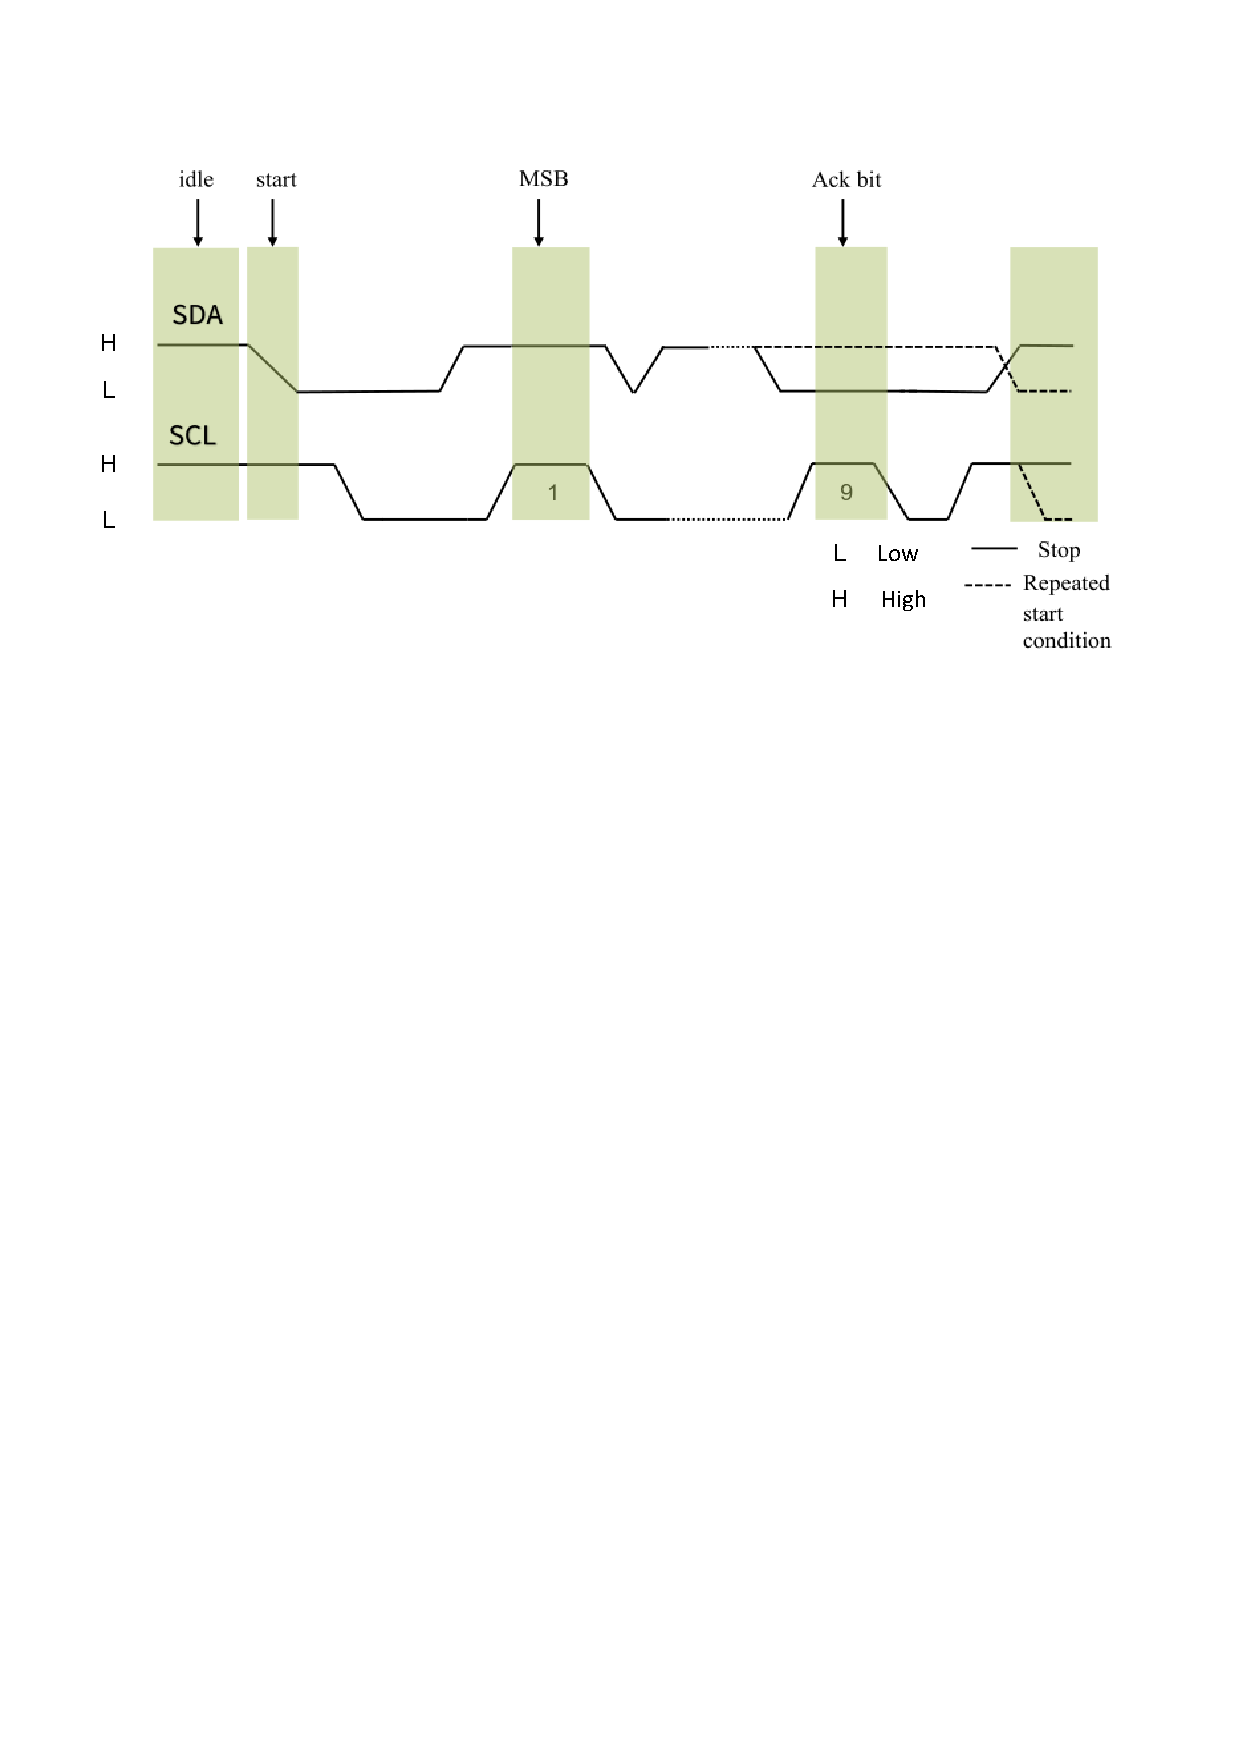
\includegraphics[trim=50 520 60 60, clip, width=140mm]{images/I2C(2).pdf}
	\caption{I2C protocol overview.}
	\label{fig:i2c_image}
\end{figure}

\begin{description}
	\item[Idle] Bus is idle when both, \Gls{SDA} and \Gls{SCL}, are inactive, i.e they are logic HIGH.
	\item[START] START condition is initiated when there is a change in the state of SDA from HIGH to LOW while SCL is still HIGH.  
	\item[Repeated START] Repeated START condition is initiated when there is a transition of SDA from HIGH to LOW while SCL is still HIGH. 
	The master uses this condition to repeat the transfer of data immediately at the end of the data transfer.
	\item[MS bit] The data that the master is intended to transfer is sent in accordance with the generation of SCL pulses. 
	The data on SDA remains unchanged during the entire high pulse of SCL; Transitions of SDA occur only during the LOW state of SCL. 
	Subsequently, data is sent to a receiving device bit wise during the rising edge of SCL.
	As shown in the \cref{fig:i2c_image}, the \Gls{MSB} of data remains unchanged during the first clock pulse of SCL, it follows that the MSB is shifted into the receiving device during the rising edge of the SCL pulse.  
	Likewise, the data is sent bit wise until the \Gls{LSB} of the data is received at the receiver. 
	\item[Acknowledge bit] For every byte data transmission, an acknowledgement bit must be received at the master.
	The master must generate a separate clock pulse associated to the reception of an acknowledgement bit. 
	\item[STOP] A STOP condition is initiated when there is a change in state of \Gls{SDA} from LOW to HIGH while \Gls{SCL} is still HIGH.
\end{description}

Using \acrshort{I2C} communication, data can be read by a master device from slave device.
DS28CM00~\cite{Maxim-DS28CM00-2006a} acts as a slave in this work.
DS28CM00 is a \acrshort{UID} chip that contains \acrshort{UID} of a slave device.
%Steps to read the UID from slave device are as follows: 
%\begin{enumerate}
%	\item Start bit is sent first.
%	\item DS28CM00 is selected as write access from master module i.e. the 8-bit slave address is sent as data using SDA line from master module.
%	 Slave address is unique for different devices. As, per the device information provided in DS28CM00 data sheet~\cite{Maxim-DS28CM00-2006a}, the slave address of the device DS28CM00 is "0xA0". 
%	In this slave address, the least significant bit is set as "0" in order to write the data onto a slave device.
%	\item Acknowledgement bit is received by master from slave, that informs about the status of the data reception.
%	\item The data containing valid memory address (between 00h and 08h) as payload is sent from master, with the direction bit set to 1.
%	The address pointer determines the location from which the master will start reading.
%	When reading from the device, the address pointer increments with every data byte read.
%	\item The repeated start condition bit is sent from master to slave to keep the bus occupied.
%	\item DS28CM00 is selected as a read access from the master module i.e the slave address along the direction bit is set to "1" in order to read the data from the slave device.
%	\item Further, to which the data is received byte-wise from master module over multiple communications. The byte-wise received data are concatenated to restore the 64-bit ROM registration number of the slave module.
%	\item The acknowledgement bits are received for every byte wise packet of ROM registration number. 
%	\item Finally, the stop condition bit is sent from master to slave, concluding the read access communication. 
%\end{enumerate}

\subsection{UDP}\label{sec:UDP}
\glsentryfull{UDP}~\cite{Tanenbaum2010} is a Transport Layer protocol~\cite{Day1983} used for low-latency connectionless communication in IP-based networks. Communication is achieved by transmitting information in the form of datagrams from source to destination without verifying the state of the receiver. 
UDP provides two services such as the port number and checksum capability. 
Port numbers are used to distinguish different user requests and checksum is an optional feature that is used to detect errors in the data that has arrived. 

\begin{figure}[hbt]
\centering
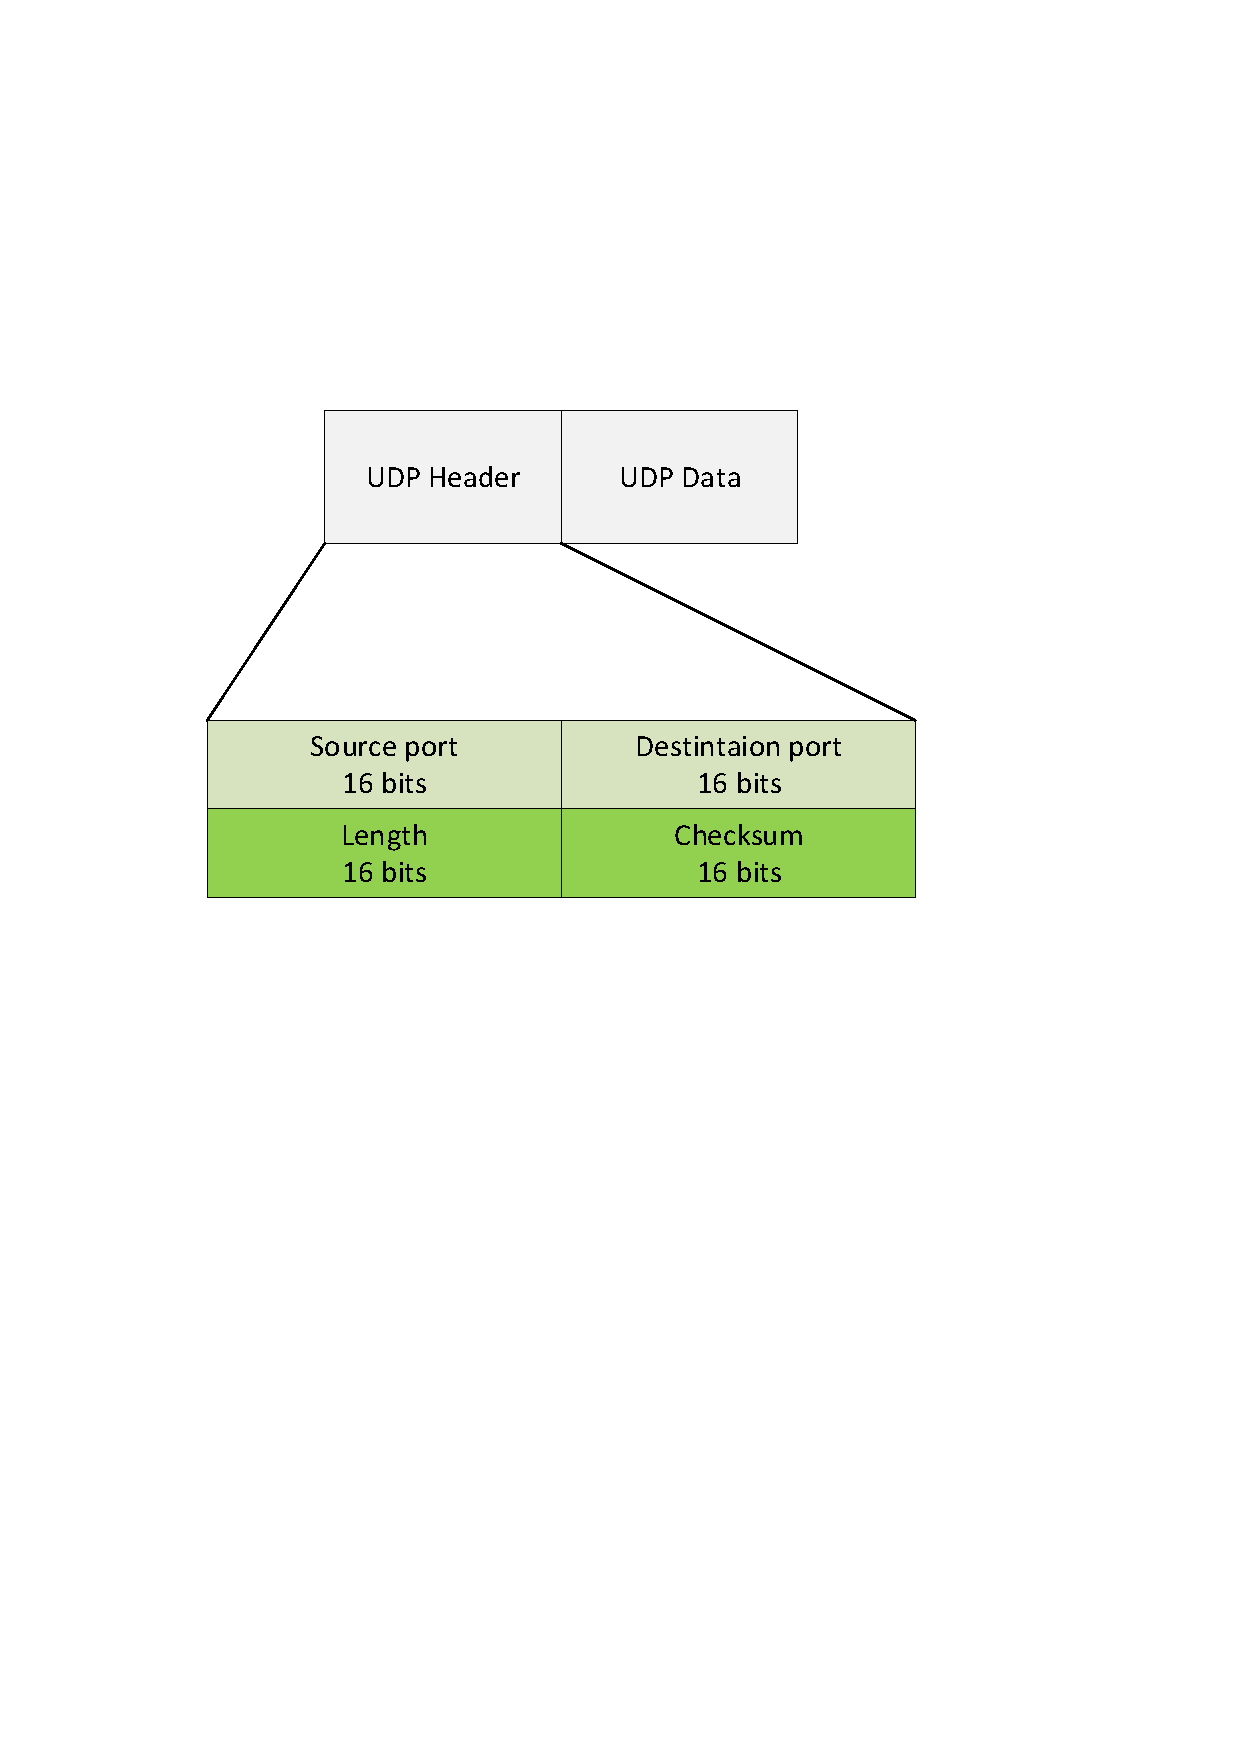
\includegraphics[trim=80 400 150 150, clip, width=80mm]{images/UDP.pdf}
\caption{User Datagram Protocol.}
\label{fig:UDP}
\end{figure}

A \acrshort{UDP} header has four fields, each of these fields is of length 2 bytes. The fields of UDP are:
\begin{itemize}[]
\item{\textbf{Source port}}: The Source port represents the port of the sender.
\item{\textbf{Destination port}}: The Destination port represents the port the datagram is addressed to.   
\item{\textbf{UDP length}}: The UDP length represents the length in bytes of the UDP header. 
\item{\textbf{Checksum}}: The Checksum is used for checking error. 
\end{itemize}

UDP, unlike other transmission protocols, does not use handshaking dialogues to provide a guarantee that data delivers to its destination. 
However, it has very low overhead. UDP works by encapsulating data inside the header field and these data are sent as packets to their destinations. 
UDP protocol is most commonly used as a basic protocol in client-server application protocols such as TFTP, DNS, etc.

\subsection{Analog-to-digital converter}\label{sec:ADC}
Analog-to-digital converter (ADC) is an electronic component~\cite{Rauth2005a} that converts an analog electrical signal (mostly voltage signal) into a digital value.  
Analog signals are the continuous-time and continuous-amplitude signals that could mean physical quantities such as sound, light, temperature, and motion.

Microcontroller consists of an ADC for the conversion of these physical quantities into digital values because microcontrollers can only work with discrete values. ADC follows certain signal processing concepts as shown in the \cref{fig:ADC} in performing the conversion of analog signals into digital values.

\begin{figure}[hbt]
\centering
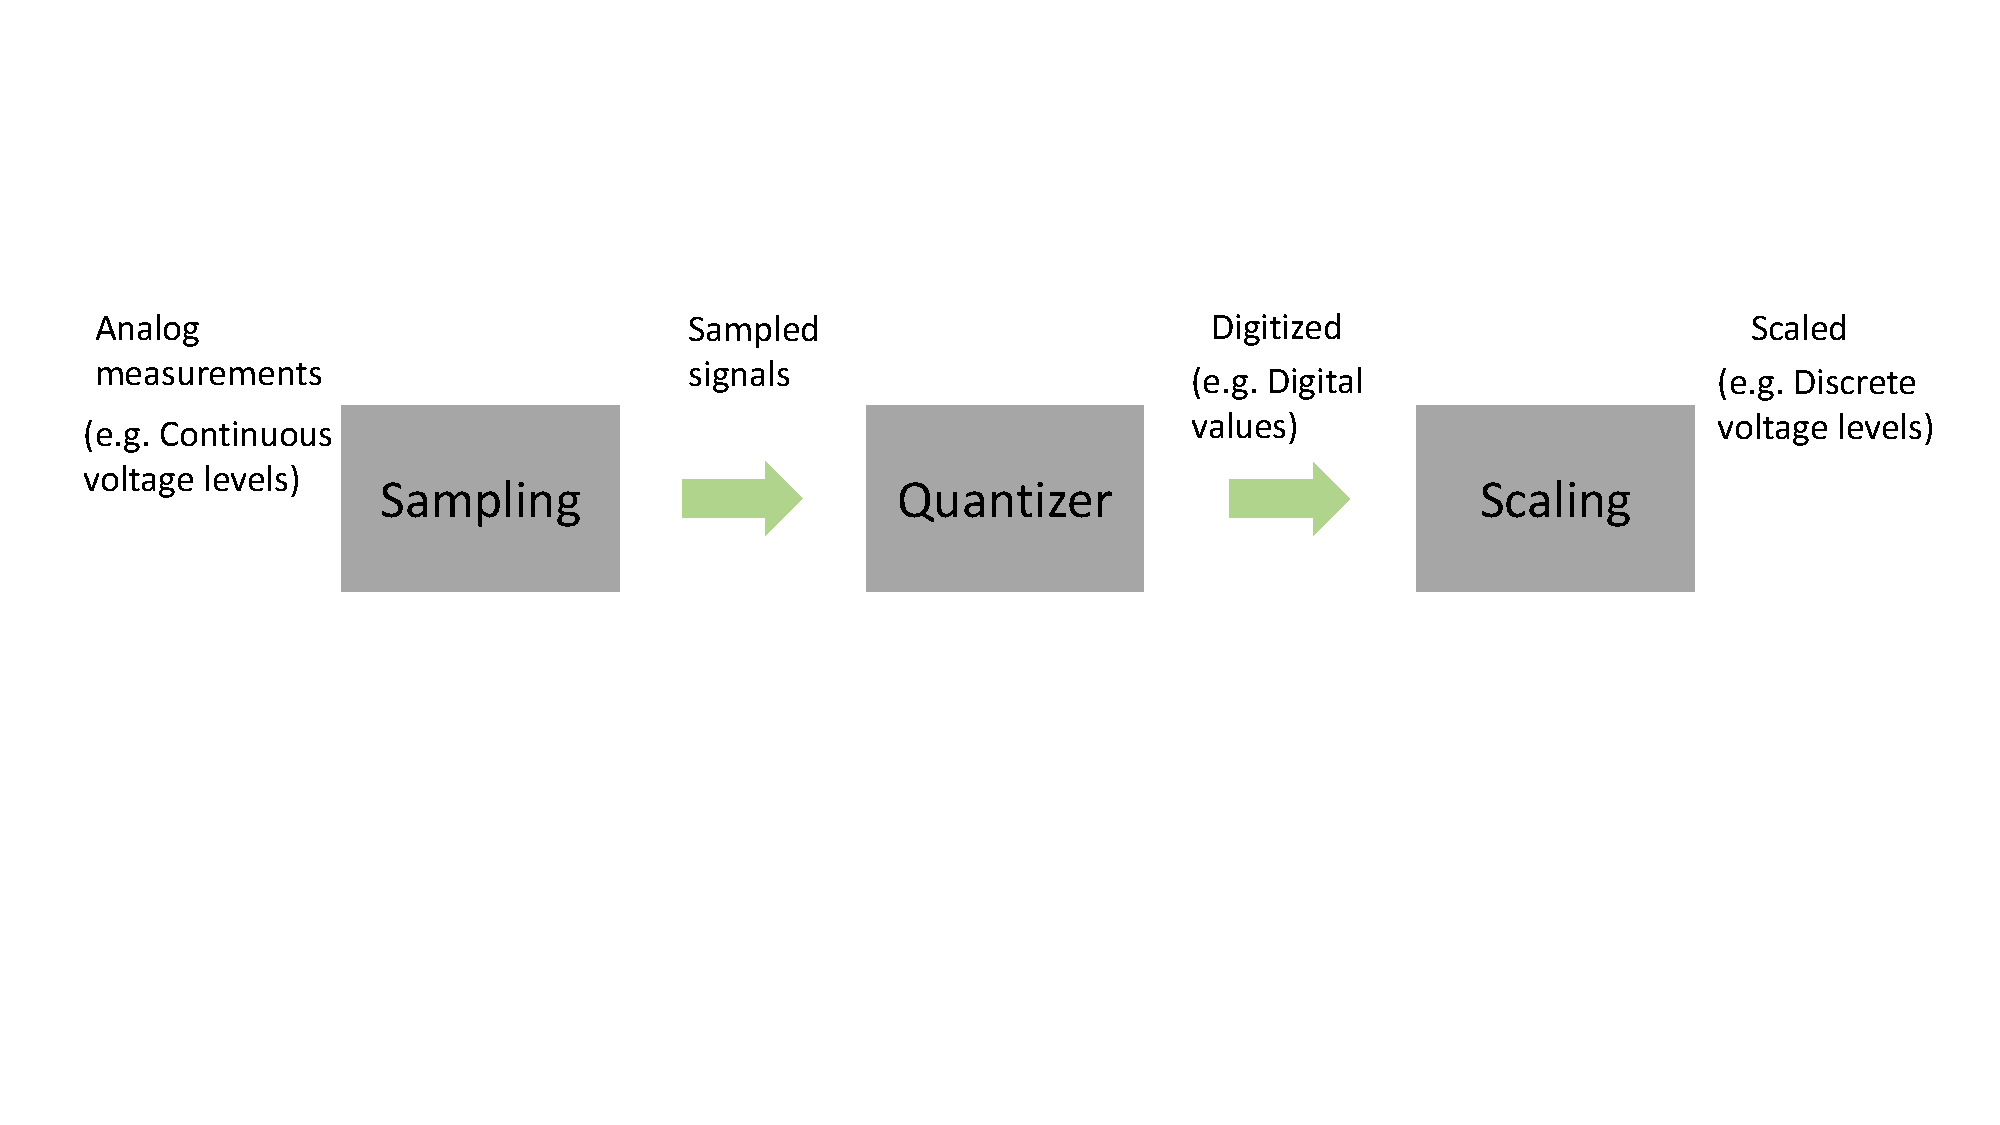
\includegraphics[trim=0 250 25 138, clip, width=150mm]{images/ADC.pdf}
\caption{Sampled Signal.}
\label{fig:ADC}
\end{figure}

\begin{description}
	\item[Signal sampling] Sampling of a signal is performed in order to reduce the continuous-time signal to a discrete-time signal where, any physical quantity such as sound wave or light wave is converted into a sequence of samples. 
	Sampling within an ADC obeys a fixed sampling rate that depends on the input signal, known as sampling frequency (${f_s}$).
	The sampled signal (see \cref{fig:Signal sampling}) is used in the digitization of its every slice. The digitization follows a fundamental principle known as the \emph{Nyquist theorem}~\cite{Miller2010a} to successfully construct a digital signal from the input signal caused by sampling. 
  According to the Nyquist theorem, the sampling frequency needs to be at least twice the highest analog frequency component (${f_{max}}$) of the input signal in order to construct a digital representation. 

The equation that represents the Nyquist criterion is given by:

${f_s} >= 2f_{max}$

  \item[Resolution] The ADC's resolution is the smallest change in voltage that can be detected and thus causes a change in the digital input. This change is also known as the step size of the ADC. The resolution (N) of the ADC can be determined by a bit length that is specific to the ADC. An ADC which has 'n' bit digital output provides $2^{n}$ digital values (resolution), i.e.,
\begin{equation}
N = 2^{n}  
\label{eq:Resolution}
\end{equation}
For example, if the digital output is of a bit length of 12-bit for an ADC, the resolution of this ADC is $2^{12}$, i.e., 4096. This also means that for ADC with the resolution 4096, the digital values for each sample of an ADC range from 0 to 4095.  
\item[Scaling] The processing of the digital data into microcontroller specific discrete voltage values is known as Scaling.
Scaling is performed by using the bit length, digital data, and reference voltage information.
  The standard scaling function of an ADC is given by:
\begin{equation}
f(x) = {\left(\dfrac{V_{max} - V_{min}}{N}\right)\cdot d} - V_{min}, \hspace{9mm}  
\label{eq:Scaling}
\end{equation}
\\
\hspace{19mm} f(x) = Scaling function,\\
\hspace{19mm} ${V_{max}}$ = Maximum analog voltage to be converted to digital output,\\
\hspace{19mm} ${V_{min}}$ = Minimum analog voltage to be converted to digital output,\\
\hspace{19mm} N = Resolution (see equation \ref{eq:Resolution}) of the ADC,\\
\hspace{19mm} d = digital value.
\end{description}
%Scaling function = \frac{V_{ref}}{d} N,


\begin{figure}[hbt]
\centering
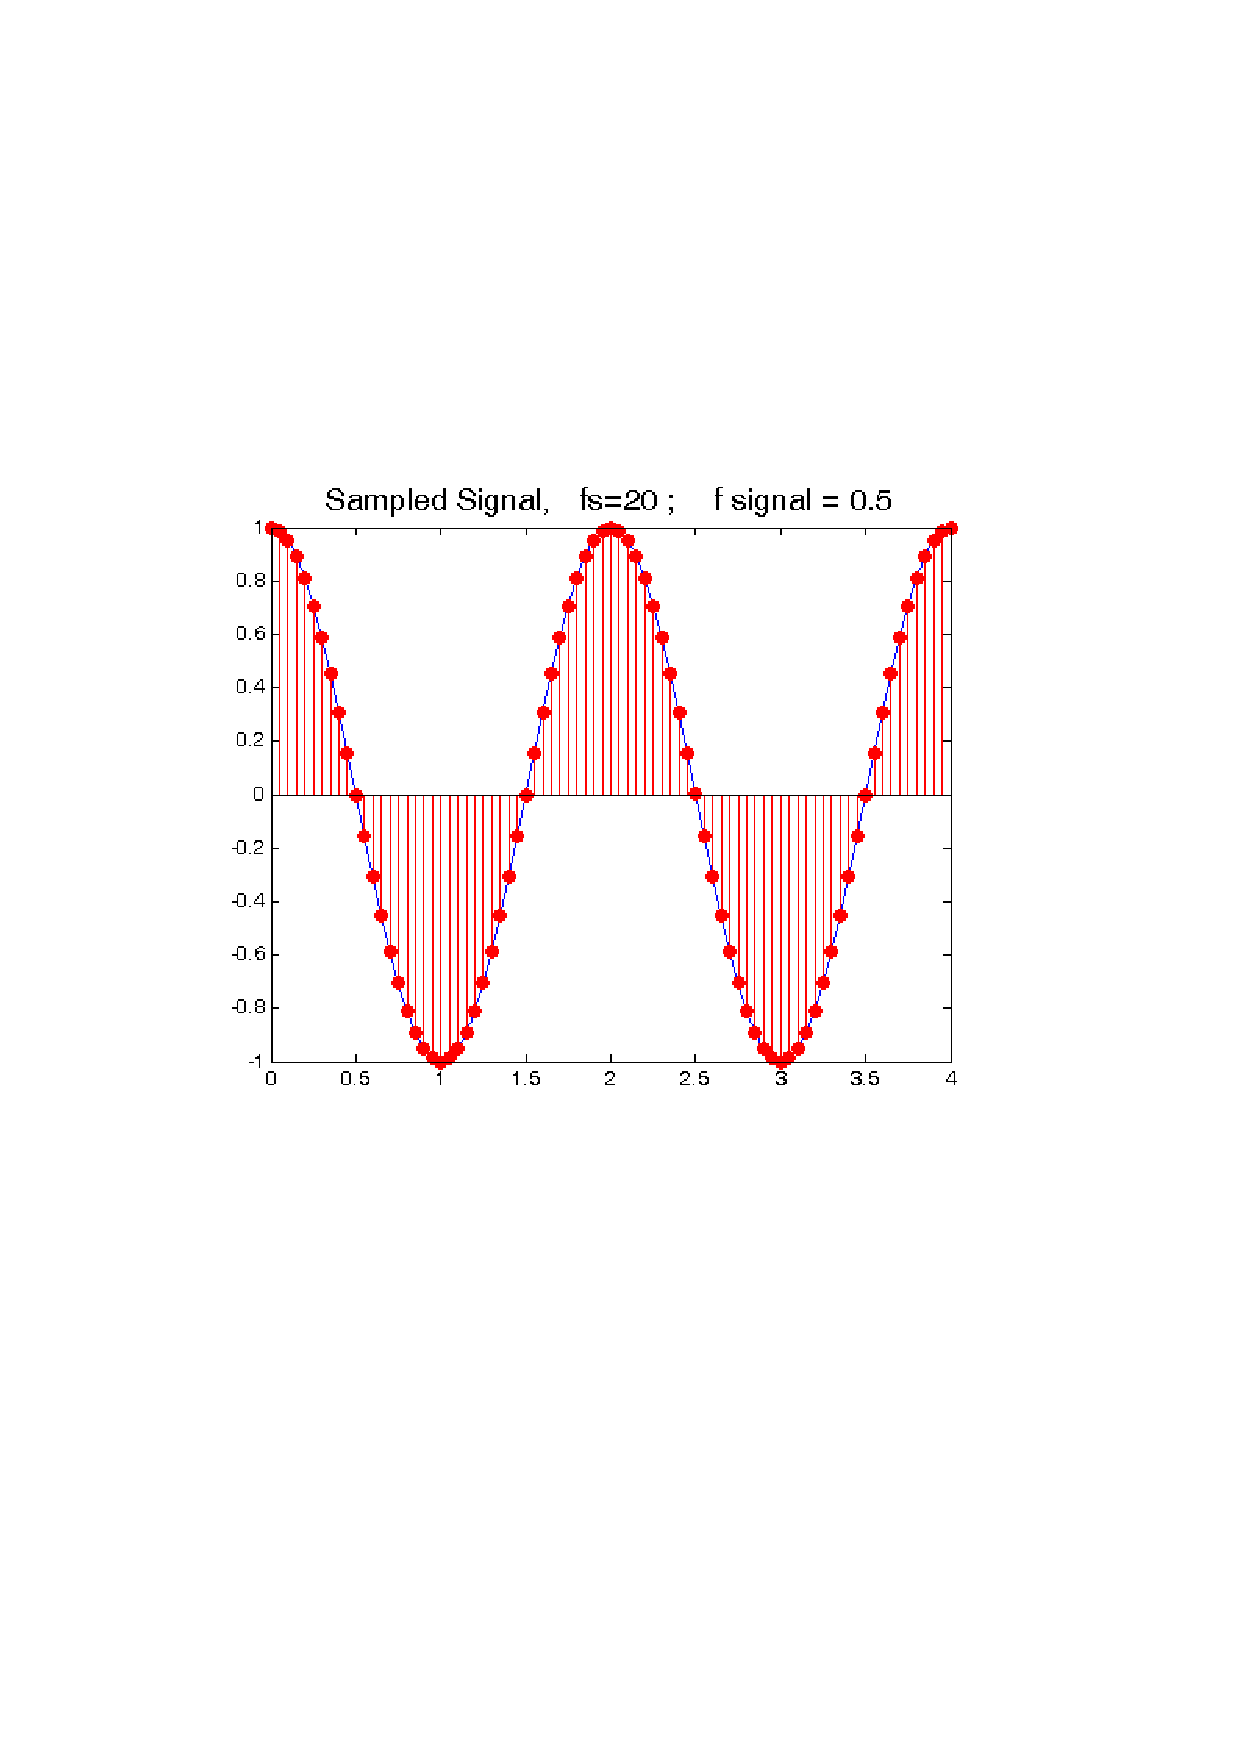
\includegraphics[trim=110 320 100 248, clip, width=80mm]{images/Sampled_signal.pdf}
\caption{Sampled Signal.}
\label{fig:Signal sampling}
\end{figure}



\section{Tools}
	\subsection{DAVE}\label{DAVE}	
			\Gls{DAVE}~\footnote{\url{https://www.infineon.com/dave}} is an Eclipse based IDE using the GNU C-compiler, designed for firmware development of ARM-based 32-bit XMC Infineon processors.
Using the C/C++ language, firmware is developed. 
			\Gls{DAVE} includes the building blocks of software development such as code editor, compiler, and debugger.
The configuration wizard of \Gls{DAVE} provides an overview over the hardware peripherals, control units, and modules. 
			\Gls{DAVE} provides a graphical user interface and wizard, which gets easy for the beginner to get acquainted with the development tool. 
			\Gls{DAVE}'s interactive user interface provides a configuration window which allows the designer to select and configure a specific product and then automatically generate system initialization code for that product, including its core, memory, peripherals, driver functions, and interrupts.    
			In \Gls{DAVE}, user-specific functionality can be added to the automatically generated code without having overwritten the parts when applying further changes to the microcontroller configurations.
%Figure to include}
	
	\subsection{Git}
		 Git~\cite{Loeliger2012a} is a distributed version control tool that supports distributed non-linear workflows. 
		 It is designed for facilitating the co-ordination between the connected programmers in developing software and, track or reverse the changes that are done in the development stages.
%Figure to include}
  		
\section{Markup languages for data interchange}
\subsection{JSON}
JSON~\cite{ECMA-404-2013} is short for JavaScript Object Notation, is a standard file format used primarily for serialization and de-serialization.
Serialization converts an Object-oriented programming's (OOP) object into a JSON string and de-serializing is to do the inverse operation.
It is represented in key-value pairs and is used widely in web applications to generate and parse data.
